\documentclass[]{elsarticle} %review=doublespace preprint=single 5p=2 column
%%% Begin My package additions %%%%%%%%%%%%%%%%%%%
\usepackage[hyphens]{url}

  \journal{NeuroImage} % Sets Journal name


\usepackage{lineno} % add
\providecommand{\tightlist}{%
  \setlength{\itemsep}{0pt}\setlength{\parskip}{0pt}}

\usepackage{graphicx}
\usepackage{booktabs} % book-quality tables
%%%%%%%%%%%%%%%% end my additions to header

\usepackage[T1]{fontenc}
\usepackage{lmodern}
\usepackage{amssymb,amsmath}
\usepackage{ifxetex,ifluatex}
\usepackage{fixltx2e} % provides \textsubscript
% use upquote if available, for straight quotes in verbatim environments
\IfFileExists{upquote.sty}{\usepackage{upquote}}{}
\ifnum 0\ifxetex 1\fi\ifluatex 1\fi=0 % if pdftex
  \usepackage[utf8]{inputenc}
\else % if luatex or xelatex
  \usepackage{fontspec}
  \ifxetex
    \usepackage{xltxtra,xunicode}
  \fi
  \defaultfontfeatures{Mapping=tex-text,Scale=MatchLowercase}
  \newcommand{\euro}{€}
\fi
% use microtype if available
\IfFileExists{microtype.sty}{\usepackage{microtype}}{}
\bibliographystyle{elsarticle-harv}
\usepackage{longtable}
\usepackage{graphicx}
% We will generate all images so they have a width \maxwidth. This means
% that they will get their normal width if they fit onto the page, but
% are scaled down if they would overflow the margins.
\makeatletter
\def\maxwidth{\ifdim\Gin@nat@width>\linewidth\linewidth
\else\Gin@nat@width\fi}
\makeatother
\let\Oldincludegraphics\includegraphics
\renewcommand{\includegraphics}[1]{\Oldincludegraphics[width=\maxwidth]{#1}}
\ifxetex
  \usepackage[setpagesize=false, % page size defined by xetex
              unicode=false, % unicode breaks when used with xetex
              xetex]{hyperref}
\else
  \usepackage[unicode=true]{hyperref}
\fi
\hypersetup{breaklinks=true,
            bookmarks=true,
            pdfauthor={},
            pdftitle={High Resolution, Unbiased CT Brain Template},
            colorlinks=false,
            urlcolor=blue,
            linkcolor=magenta,
            pdfborder={0 0 0}}
\urlstyle{same}  % don't use monospace font for urls

\setcounter{secnumdepth}{5}
% Pandoc toggle for numbering sections (defaults to be off)

\newlength{\cslhangindent}
\setlength{\cslhangindent}{1.5em}
\newenvironment{cslreferences}%
  {\setlength{\parindent}{0pt}%
  \everypar{\setlength{\hangindent}{\cslhangindent}}\ignorespaces}%
  {\par}

% Pandoc header
\usepackage{booktabs}
\usepackage{longtable}
\usepackage{array}
\usepackage{multirow}
\usepackage{wrapfig}
\usepackage{float}
\usepackage{colortbl}
\usepackage{pdflscape}
\usepackage{tabu}
\usepackage{threeparttable}
\usepackage{threeparttablex}
\usepackage[normalem]{ulem}
\usepackage{makecell}
\usepackage{xcolor}



\begin{document}
\begin{frontmatter}

  \title{High Resolution, Unbiased CT Brain Template}
    \author[JHSPH]{John Muschelli}
   \ead{jmusche1@jhu.edu} 
      \address[JHSPH]{Johns Hopkins Bloomberg School of Public Health, Department of Biostatistics, 615 N Wolfe St, Baltimore, MD, 21205}
    
  \begin{abstract}
  Clinical imaging relies heavily on X-ray computed tomography (CT) scans for diagnosis and prognosis. Many research applications aim to perform population-level analyses, which require images to be put in the same space, usually defined by a population average, also known as a template. We present an open-source, publicly available, high-resolution CT template. With this template, we provide voxel-wise standard deviation and median images, a basic segmentation of the cerebrospinal fluid spaces, including the ventricles, and a coarse whole brain labeling. This template can be used for spatial normalization of CT scans and research applications, including deep learning. The template was created using an anatomically-unbiased template creation procedure, but is still limited by the population it was derived from, an open CT data set without demographic information. The template and derived images are available at https://github.com/muschellij2/high\_res\_ct\_template.
  \end{abstract}
  
 \end{frontmatter}

\hypertarget{introduction}{%
\section{Introduction}\label{introduction}}

Many research applications of neuroimaging use magnetic resonance imaging (MRI). MRI allows researchers to study a multitude of applications and diseases, including studying healthy volunteers as it poses minimal risk. Clinical imaging, however, relies heavily on X-ray computed tomography (CT) scans for diagnosis and prognosis. Studies using CT scans cannot generally recruit healthy volunteers or large non-clinical populations due to the radiation exposure and lack of substantial benefit. As such, much of head CT data is gathered from prospective clinical trials or retrospective studies based on health medical record data and hospital PACS (picture archiving and communication system). Most of this research is on patients with neuropathology, which can cause deformations of the brain, such as mass effects, lesions, stroke, or tumors.

Many clinical protocols perform axial scanning with a high within-plane resolution (e.g.\(0.5\)mm x \(0.5\)mm) but lower out-of-plane resolution (e.g.~\(5\)mm). High resolution scans (out of plane resolution \(\approx 0.5\)mm) may not be collected or reconstructed as the lower resolution scans are typically those read by the clinician or radiologist for diagnosis and prognosis. Recently, a resource of a large number of CT scans were made available, denoted as CQ500 (Chilamkurthy et al. 2018). These scans include people with a number of pathologies, including hemorrhagic stroke and midline shifts. Fortunately, this data also includes people \textbf{without indicated pathology} with high resolution scanning, which is what we will use in this study.

The goal of this work is to create an anatomically unbiased, high-resolution CT template of the brain. That is, we wish to create a template that represents the population, regardless of any initial templates we start with. The first, and we believe the only, publicly-available CT template was released by Rorden et al. (2012) (https://www.nitrc.org/projects/clinicaltbx/). That template was created with the specific purpose of creating a template with a similar age range as those with stroke, using 30 individuals with a mean age of 65 years old (17 men). The associated toolbox released contained a high resolution (1x1x1mm) template, with the skull on, in Montreal Neurological Institute (MNI) space. Subsequent releases have included skull-stripped brain templates, but only in a lower (2x2x2mm) space (https://github.com/neurolabusc/Clinical). This lower resolution template matches what is used in many MRI and functional MRI analyses.

Thus, the current CT templates available are a high-resolution template (1mm\(^3\)), but not of the brain only (and skull stripping the template performs marginally well), and a low-resolution template of the brain only, both in MNI space. We have used these templates in previous analyses, but would like a brain template that was 1) constructed using an unbiased anatomical procedure, 2) uses more patients, 3) uses high-resolution scans to achieve a higher resolution, and 4) provide an image which dimensions are easily used in deep learning frameworks.

As the CQ500 data was released under a Creative Commons Attribution-NonCommercial-ShareAlike 4.0 (CC-NC-SA) International License, we can release the template under the same license.

\hypertarget{methods}{%
\subsection{Methods}\label{methods}}

All code, analysis, and reporting was done the R statistical programming language (R Core Team 2015) and a number of packages from the R medical imaging package platform Neuroconductor (Muschelli et al. 2019).

\hypertarget{data}{%
\subsubsection{Data}\label{data}}

We defined a high-resolution patient scan as having a within-axial resolution of \(0.7\)x\(0.7\)mm or less, with full coverage of the brain. For example, if the cerebellum was not imaged, that image was discarded. All scans were non-contrast CT scans with a soft-tissue convolution kernel. As CT scans are generally well calibrated across sites and are measured in standard units of Hounsfield Units (HU), no intensity normalization was done. Intensities less than \(-1024\) HU (the value for air) and greater than \(3071\) HU were Winsorized to those values, as values outside of these are likely artifact or areas outside the field of view.

All data was converted from DICOM files to NIfTI (Neuroimaging Informatics Technology Initiative) using \texttt{dcm2niix} (Li et al. 2016) using the \texttt{dcm2niir} package (Muschelli 2018). This conversion corrects for any gantry tilt and enforces one fixed voxel size for the image, which is necessary if different areas of the image are provided at different resolutions, which is sparsely seen in clinical CT images.

From the CQ500 data set, 222 subjects had no indication of pathology, of which 141 had a high-resolution scan (if multiple were present, the one with the highest resolution was used). From these 141 people, 130 had ``thick-slice'' scans where the out-of-plane resolution was greater than \(4\)mm. We used these 130 scans for construction of the template. The 11 scans were discarded as we wish to perform the same operation using low-resolutions scans to see the effect of initial resolution on template creation, but that is not the focus of this work.

For all images, the head was skull-stripped so that only brain tissue and cerebrospinal fluid (CSF) spaces were kept, using a previously validated method (Muschelli et al. 2015) using the brain extraction tool (BET) from FSL (FMRIB Software Library
) (Smith 2002; Jenkinson et al. 2012). We chose an image (patient 100 from CQ500), for template creation. This choice was based on a within-plane resolution close to \(0.5\)x\(0.5\)mm (\(0.488\)x\(0.488\)mm), an axial slice size of 512x512, and an out-of-plane resolution of \(0.5\)mm. The image was resampled to \(0.5\)x\(0.5\)x\(0.5\)mm resolution so that the voxels are isotropic. We would like the image to be square; we padded the image back to 512x512 after resampling, and the image had 336 coronal-plane slices.

\hypertarget{template-creation}{%
\subsubsection{Template Creation}\label{template-creation}}

The process of template creation can be thought of as a gradient descent algorithm to estimate the true template image as inspired by the advanced normalization tools (ANTs) software and the R package ANTsR that implements the registration and transformation was used (https://github.com/ANTsX/ANTsR). The process is as follows:

\begin{enumerate}
\def\labelenumi{\arabic{enumi}.}
\tightlist
\item
  Let \(I_{i}\) represent the image where \(i\) represents subjects. We registered all images to the template, denoted \(\bar{T}_{k}\) where \(k\) represents iteration, using an affine registration followed by symmetric normalization (SyN), a non-linear deformation/diffeomorphism, where the composed transformation is denoted as \(G_{i, k}\) (Avants et al. 2008). Let the transformed image be denoted as \(T_{i, k}\). In other words, \(I_{i}\overset{G_{i,k}}{\rightarrow}T_{i, k}\). The transformation \(G_{i, k}\) is represented by a 4D warping image. Let \(T_{1}\) be the original template chosen above and \(G_{i, 1}\) be the transformation for an image to the original template.
\item
  Calculate a the mean, median, and standard deviation images, where the mean image is \(\bar{T}_{k} = \frac{1}{n} \sum\limits_{i = 1}^n T_{i, k}\), using a voxel-wise average.\\
\item
  Calculate the average warping transformation: \(\bar{G}_{k} = \frac{1}{n} \sum\limits_{i = 1}^n G_{i, k}\). A gradient descent step size of 0.2 was specified for SyN gradient descent, such that:
  \(\bar{T}_{k + 1} = \bar{T}_{k} \times \left(-0.2 * \bar{G}_{k}\right)\). The median and standard deviation are transformed accordingly.
\end{enumerate}

For each iteration \(k\), we can calculate a number of measures to determine if the template has converged compared to the previous iteration \(k - 1\). We calculated the Dice Similarity Coefficient (DSC) between the mask of iteration \(k\) and \(k-1\), where the mask for iteration \(k\) is defined as \(\bar{T}_{k} > 0\). The DSC measures if the overall shape is consistent across iterations. We also the root mean squared error (RMSE) of voxel intensities, e.g.~\(\frac{1}{V} \sum\left(\bar{T}_{k} - \bar{T}_{k-1}\right)^2\), where \(V\) is the number of voxels in the volume. The RMSE can be calculated over a series of volumes, either 1) the entire image, 2) over the non-zero voxels in iteration \(k\), 3) in iteration \(k-1\), or 4) the union (or intersection) of the 2 masks. Calculation over the entire image gives an optimistic estimate as most of the image are zeroes, and the choice of either iteration \(k\) or \(k-1\) masks is arbitrary, so we calculated the RMSE over the union of the 2 masks. The RMSE represents if the values of the image are close across iterations.

To define convergence, we would like a high DSC between the masks and a low RMSE. Ideally, the convergence criteria would set a DSC of \(1\) and a RMSE less than \(1\) Hounsfield Unit (HU), which would indicate the voxel intensity is changing less than \(1\) HU on average. As CT scans are measured in integers, this RMSE would likely be as good as possible. We set a DSC cutoff of \(0.95\) and chose the template with the lowest RMSE. As this procedure is computationally expensive, we ran \(40\) iterations, which was adequate for achieving stable results (Figure \ref{fig:performance}).

Values of the final template that were lower than \(5\) HU were boundary regions, outside the region of the brain and likely due to average of one or a small few of images, incongruent with the remainder of the template (Supplemental Figure \ref{fig:boundary}). We did not constrain the DSC and RMSE calculation excluding these regions, but excluded values less than \(5\) HU from the final template.

After the template was created, we padded the coronal plane so that the template was 512x512x512. The intention is that these dimensions allow it easier to create sub-sampled arrays that are cubes and multiples of 8, such as 256x256x256, 128x128x128, or 64x64x64 with isotropic resolution.

\hypertarget{segmentation}{%
\subsubsection{Segmentation}\label{segmentation}}

Though the template itself is the main goal of the work, many times researchers use or are interested in annotations/segmentations of the template space. The contrast between gray matter and white matter in CT imaging is not as high as T1-weighted MRI. Some areas, such as the cerebellum, corpus callosum, and basal ganglia can be delineated well. Thus, segmentation methods based on intensity may not differentiate gray and white matter adequately. We instead used a multi-atlas registration approach using previously-published set of 35 MRI atlases from Landman et al. (2012), which had whole brain segmentations, including tissue-class segmentations.

We registered each brain MRI to the CT template using SyN and applied the transformation to the associated tissue segmentation and whole brain segmentation from that MRI template. Thus, we had 35 tissue segmentations of the CT template in template space, and the segmentations were combined using STAPLE (Warfield, Zou, and Wells 2004) via the \texttt{stapler} package (Muschelli 2019). The whole brain structures were combined using majority vote.

Separating the brain from the cerebrospinal fluid areas (mainly ventricles) are of interest in many applications, such as Alzheimer's disease {[}Leon et al. (1989); braak1999neuropathology{]}. In addition, we segmented the template using Atropos (Avants et al. 2011), which used a k-means clustering approach with 2 clusters (CSF/tissue) to obtain a CSF mask. Additionally, we registered the MNI T1-weighted template to the CT Template using SyN, and applied the transofrmation used the ALVIN (Automatic Lateral Ventricle delIneatioN) mask of the ventricles (Kempton et al. 2011). We masked the CSF mask with this transformed ALVIN mask to get a mask of lateral ventricles as well.

\hypertarget{results}{%
\subsection{Results}\label{results}}

As we see in Figure \ref{fig:performance}A, the DSC quickly increases and reaches a high score, where the horizontal line indicates a DSC of \(0.99\). The red dot and vertical line indicate the iteration that had the maximum DSC (0.9896). As the DSC is high for all iterations past iteration \(15\), we chose the template based on the minimum RSE. In Figure \ref{fig:performance}B, we see a similar pattern of improving performance, but by lowering the RMSE. The lowest RMSE is noted by the red point with a value of \(1.47\). Thus, this iteration (iteration \(37\)) is the template we will choose.

\begin{figure}
\centering
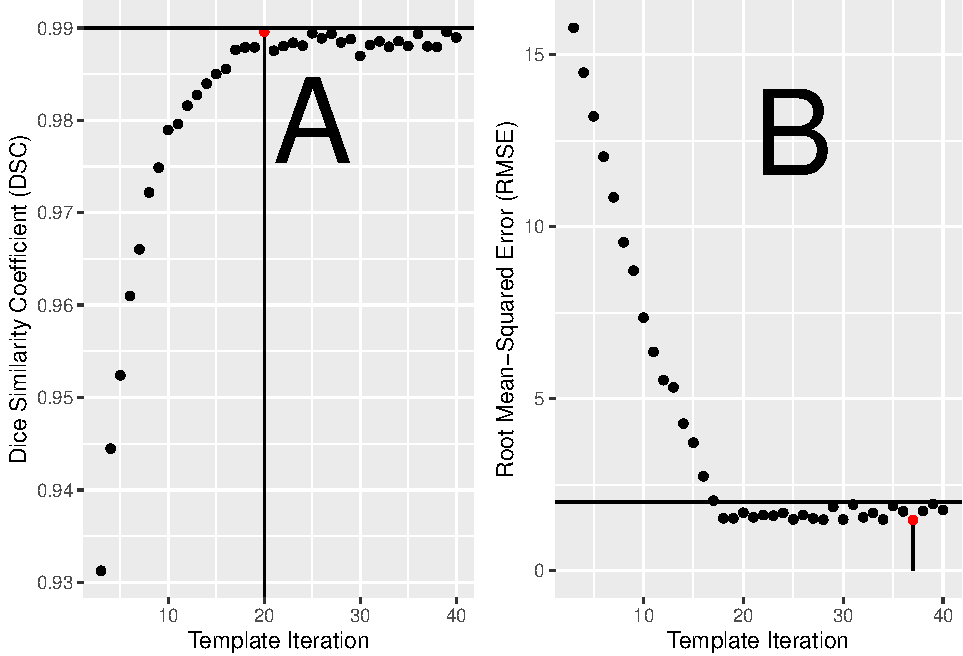
\includegraphics{index_files/figure-latex/performance-1.pdf}
\caption{\label{fig:performance}Convergence of Shape and Intensity of the Template over Iterations. Here we see the Dice Similarity Coefficient (DSC) increase between an iteration and the previous iteration, achieving high degrees of overlap, indicating the shape of the surface of the image is similar and converging (panel A). We also see the root mean-squared error (pane) drops as the iterations increase and then levels off around 4 Hounsfield units (HU), the horizontal line. The red dot indicates the iteration chosen for the template.}
\end{figure}

\begin{figure}
\centering
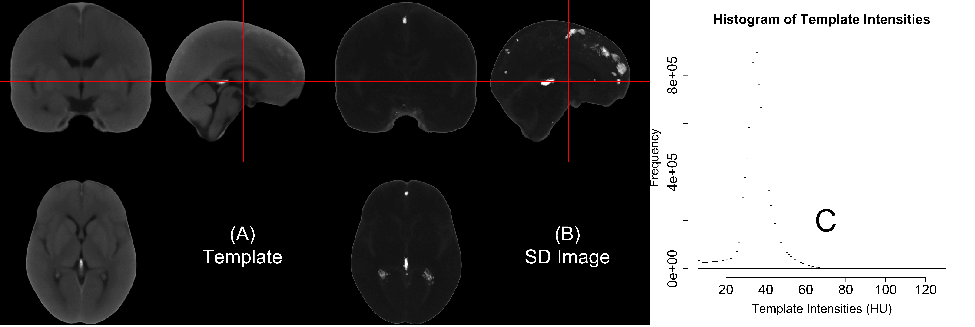
\includegraphics{index_files/figure-latex/template-1.pdf}
\caption{\label{fig:template}Template Image, Standard Deviation Image, and Histogram of Intensities. Here we show the template in the left panel, the voxel-wise standard deviation, denoting areas of variability (which include biological and technical variability), and the histogram of the template intensities/Hounsfield Units (HU). Overall the template is smooth and values fall in the range of 5 to 65 HU.}
\end{figure}

The template for this image can be seen in Figure \ref{fig:template}, along with the standard deviation image, and a histogram of the intensities of the template. Areas outside the brain mask were removed for visualization. We see the template is relatively smooth, with values from 5 HU to around 65 HU. The standard deviation image shows high variability around the lateral horns, which may be due to calcifications in a set of patients, which have abnormally high HU values. The high standard deviation areas near the midline are likely due to dense areas of the falx cerebri, including potential falx calcifications.

\begin{figure}
\centering
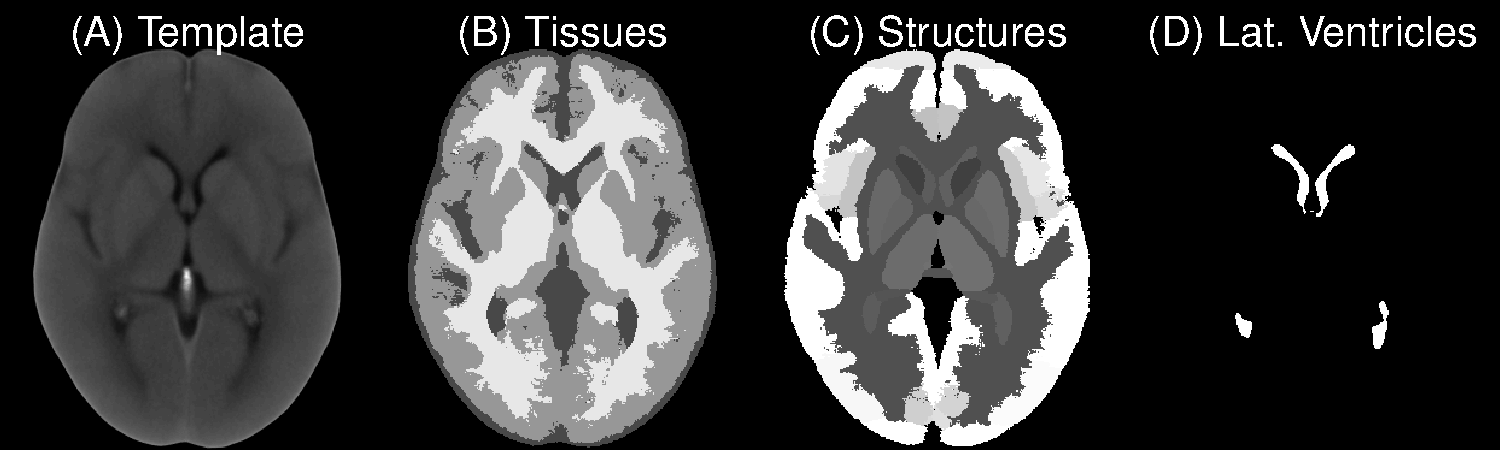
\includegraphics{index_files/figure-latex/all_segs.pdf}
\caption{\label{fig:seg}Template Image, Tissue Segmentation, Whole Brain Segmentation, and Lateral Ventricle Segmentation. We see the areas of white matter, gray matter, cebebrospinal fluid (CSF) in Panel B. We see the whole brain structural segmentation in Panel C, and the lateral ventricle segmentation from Atropos in Panel D.}
\end{figure}

In Figure\ref{fig:seg}, we see the template again, with the tissue-class segmentation (Panel B), whole brain structural segmentation (Panel C), and Atropos lateral ventricle segmentation. Overall, we see some differences between the segmentation of the CSF based on Atropos and the multi-atlas labeling approach. We have provided a lookup table for each structure label with its corresponding value in the image.

\hypertarget{discussion}{%
\subsection{Discussion}\label{discussion}}

We present a high-resolution, publicly-available CT template with associated segmentations and other annotations of the template. The data used was from a publicly-available dataset, the CQ500. The main downside with the CQ500 data set is that no demographic or clinical information was released for each patient, save for indication for pathology. Therefore, we cannot attest the general population of interest for this template. Furthermore, we cannot fully assume these patients were disease-free as a lack of pathology only applies to the categories of interest in the CQ500 dataset (intracranial/subdural/subarachnoid/epidural hematoma, calvarial or other fractures, mass effect and midline shifts). In future work, we hope to prepare age- and sex-specific templates for each population based on hospital scans and records, where we have demographic information and confirmation of lack of neuropathology.

In addition to the template, we have provided a set of segmentations. This includes a whole brain segmentation of over 150 structures. Though this may prove useful, we caution users to how well this template can provide an accurate segmentation of these structures. At least, the accuracy of the segmentation may have variable accuracy at different areas of the brain.

The resulting image dimensions was 512x512x512, with a resolution of 0.5x0.5x0.5mm. The fact that the image dimension is a multiple of 8 allows it to be resampled to 1x1x1mm and 2x2x2mm and remain as a cube. These dimensions are particularly important in certain deep learning architectures and frameworks. Though most templates are given using the mean image, we believe the standard deviation image represents variability in the area. This variability represents true systematic and biologic variability. One important area of systemic variability is registration errors. Therefore this template allows for the creation of z-score images, where a new image is registered to the mean image, the mean image is subtracted, and then divided by the standard-deviation image, so that voxels represent standard deviations away from the mean voxel. This image may be a useful tool in feature extraction. Thus, we believe this template provides a standard, isotropic space that is conducive to machine learning and can reduce the burden of standardization for medical imaging applications.

CQ500 is Creative Commons Attribution-NonCommercial-ShareAlike 4.0 International License. Therefore, the template is released under the same license. The images are located on https://github.com/muschellij2/high\_res\_ct\_template and can be accessed at https://johnmuschelli.com/high\_res\_ct\_template/template/.

\hypertarget{acknowledgments}{%
\subsection{Acknowledgments}\label{acknowledgments}}

This work has been been supported by the R01NS060910 and 5U01NS080824 grants from the National Institute of Neurological Disorders and Stroke at the National Institutes of Health (NINDS/NIH).

\hypertarget{references}{%
\section*{References}\label{references}}
\addcontentsline{toc}{section}{References}

\hypertarget{supplemental-material}{%
\section{Supplemental Material}\label{supplemental-material}}

In Supplemental Figure \ref{fig:boundary}, we show the voxels in the template that had values less than 5 Hounsfield units. We removed these voxels from the final template as they are likely voxels from only a few subjects.

\begin{verbatim}
## pdf 
##   2
\end{verbatim}

\begin{figure}
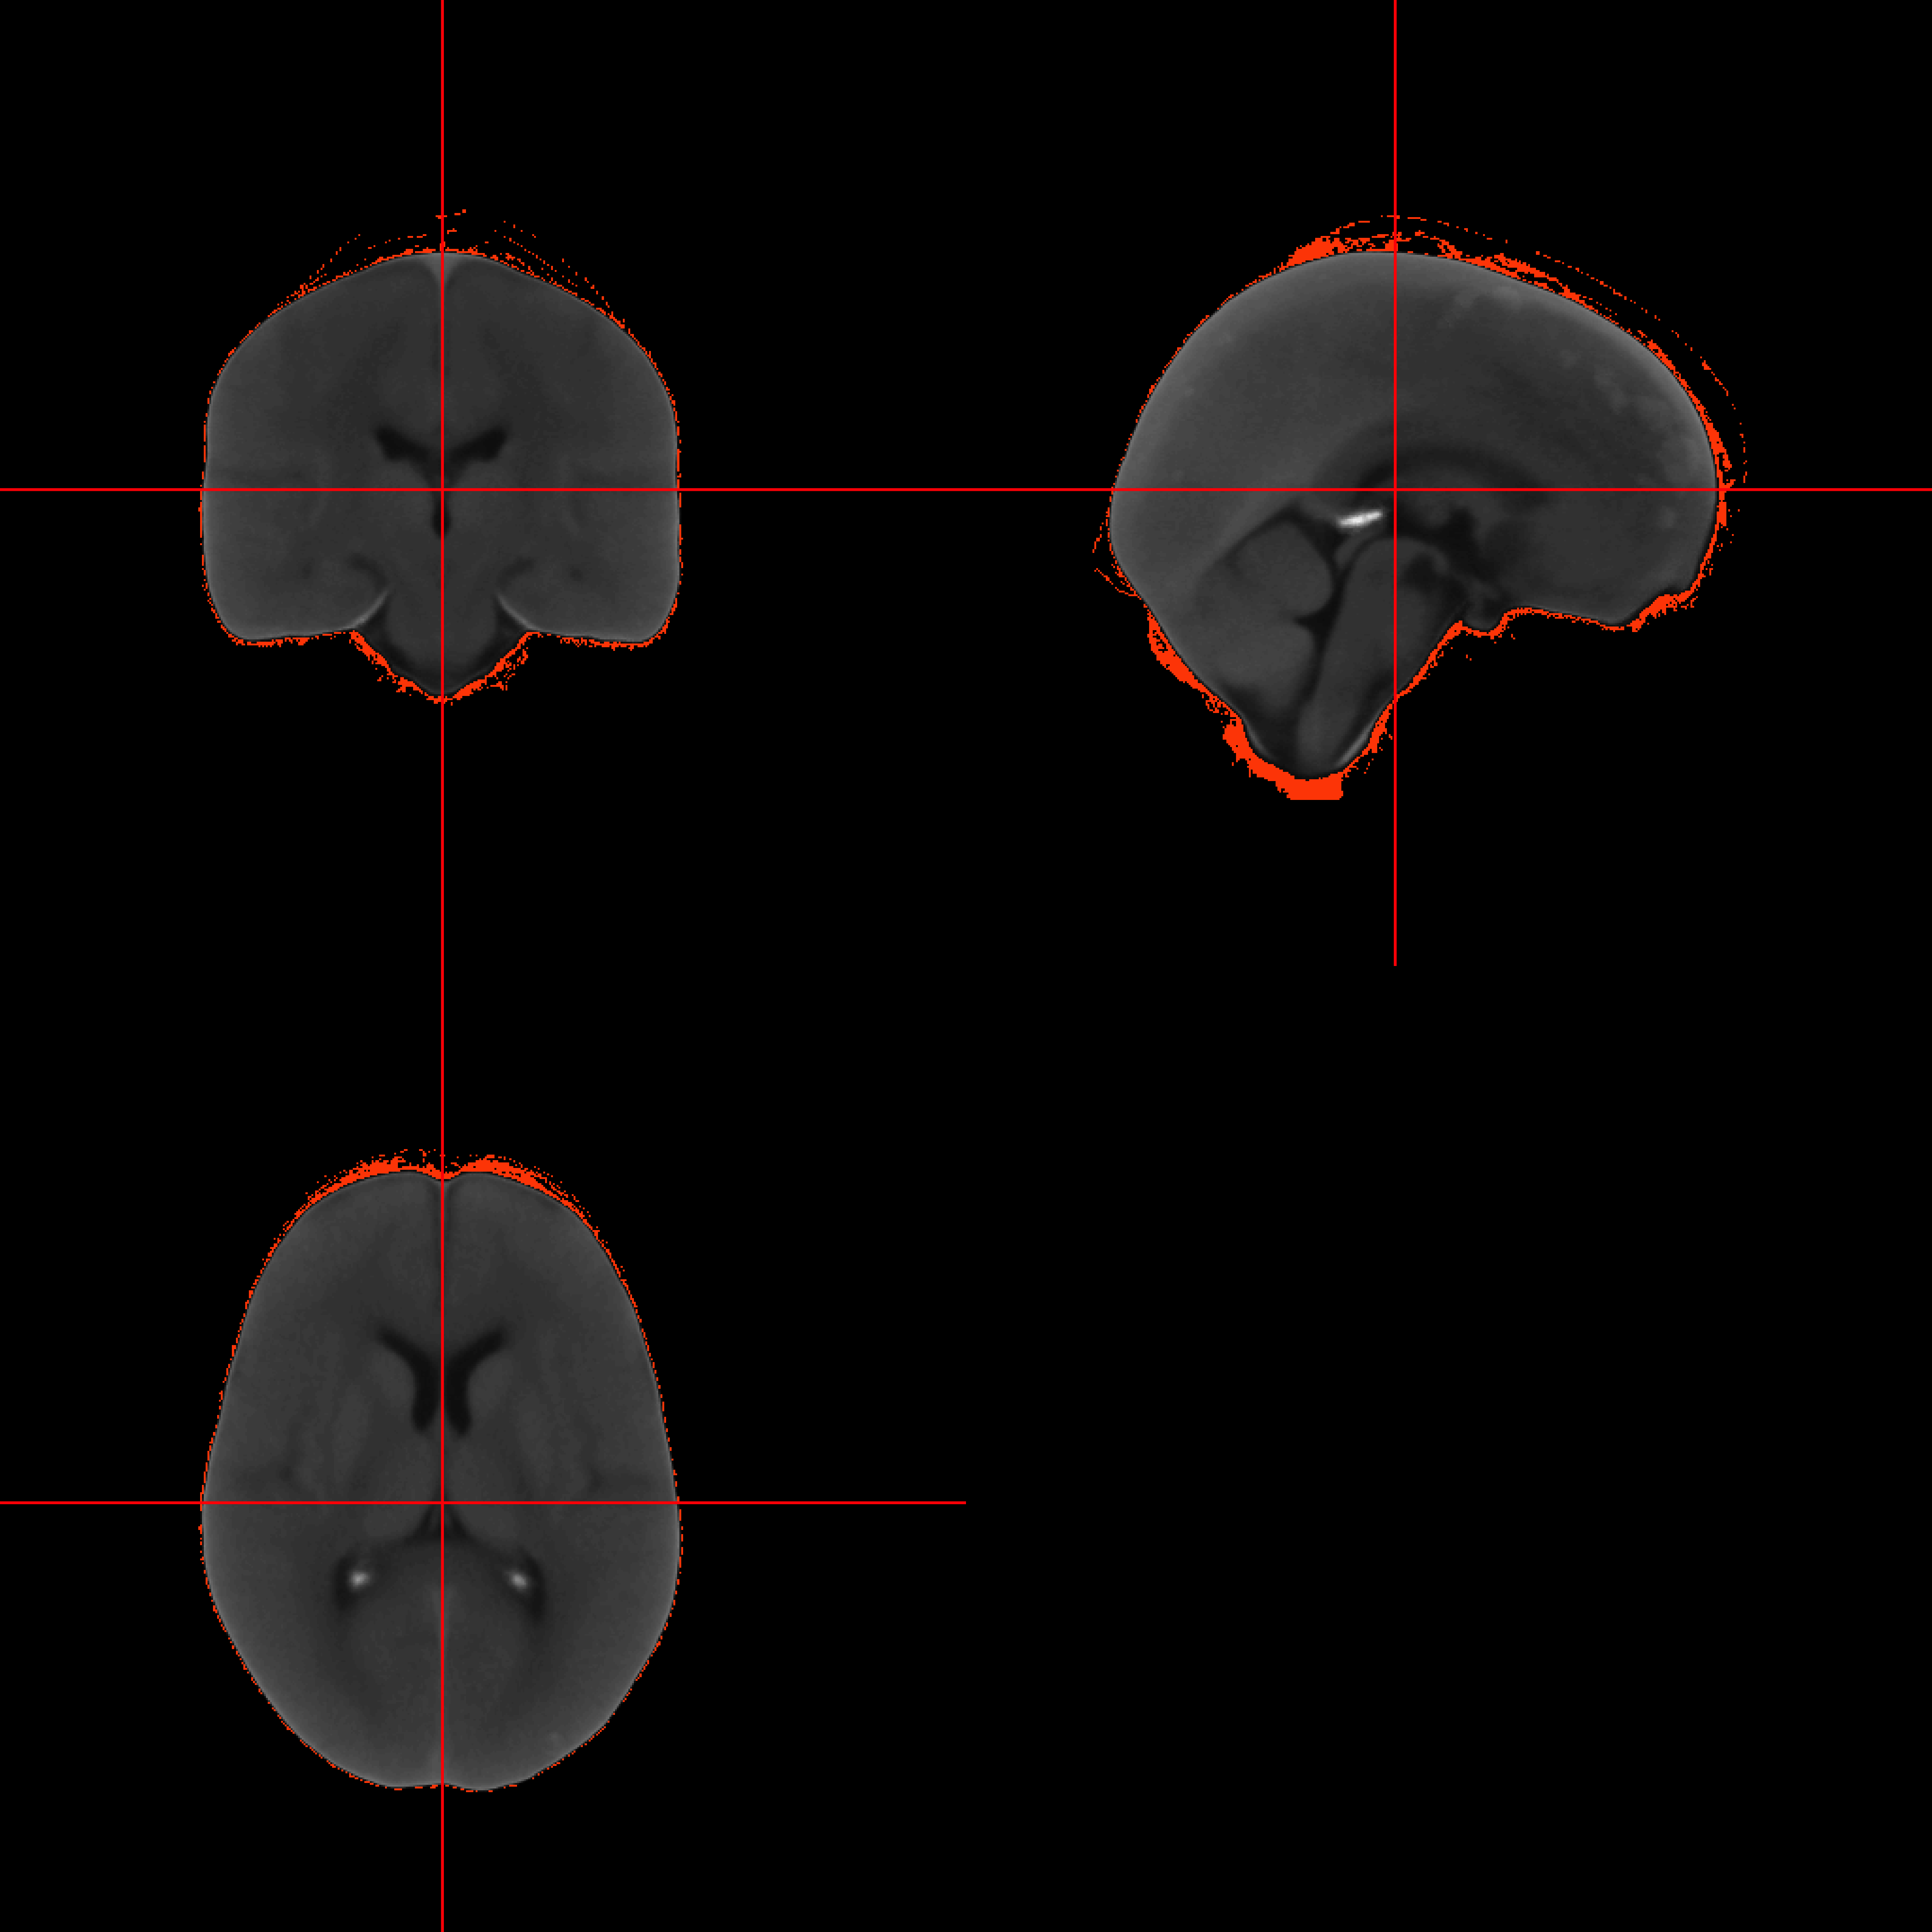
\includegraphics[width=1\linewidth]{index_files/figure-latex/sd_image} \caption{Boundary Issues with Low HU Values.  Here we present the average image with the mask of voxels that were lower than 5 HU in the template.  We excluded these values from the final template.}\label{fig:boundary}
\end{figure}

In Supplemental Figure \ref{fig:median} we show the template image, but using the voxel-wise median rather than the mean. We see fewer areas of high intensity, as the median is resistant to large outliers. We do see some brighter areas towards the cortical surface, which may be a byproduct of partial voluming effects with the skull or truly denser areas.

\begin{figure}
\centering
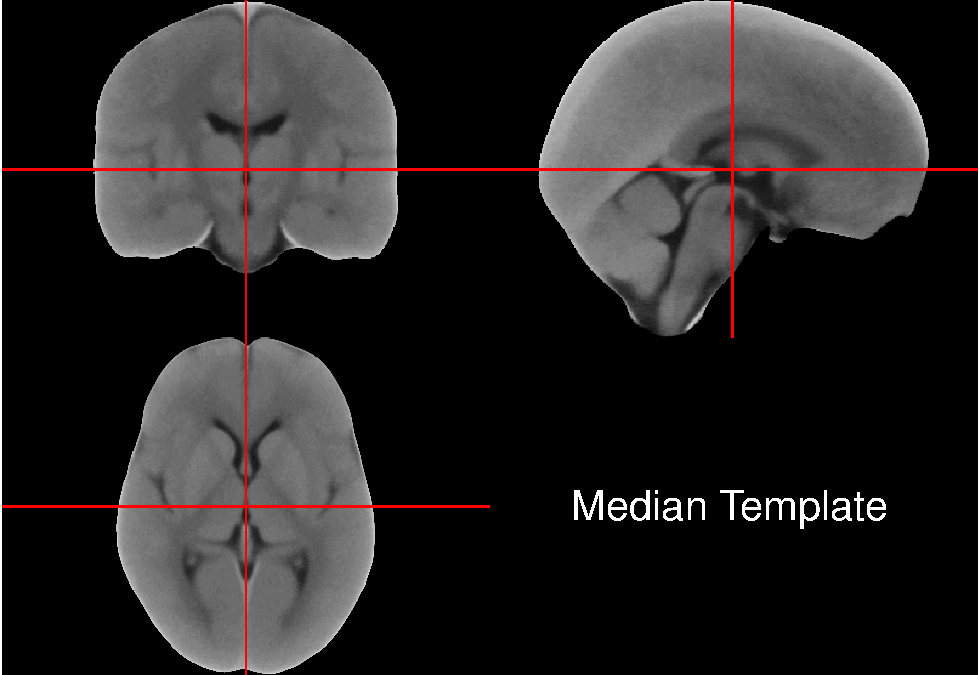
\includegraphics{index_files/figure-latex/median-1.pdf}
\caption{\label{fig:median}Median Image. We see fewer areas of high intensity, as the median is resistant to large outliers. We do see some brighter areas towards the cortical surface, which may be a byproduct of partial voluming effects with the skull or truly denser areas.}
\end{figure}

In Supplemental Table \ref{tab:labs} Here we present a set of the labels for the structures in the structural segmentation of the template.

\begin{table}

\caption{\label{tab:labs}Example Structure Labels.  Here we present a set of the labels for the structures in the structural segmentation of the template.}
\centering
\begin{tabular}[t]{r|l}
\hline
index & name\\
\hline
50 & Left Inf Lat Vent\\
\hline
51 & Right Lateral Ventricle\\
\hline
52 & Left Lateral Ventricle\\
\hline
53 & Right Lesion\\
\hline
54 & Left Lesion\\
\hline
55 & Right Pallidum\\
\hline
56 & Left Pallidum\\
\hline
57 & Right Putamen\\
\hline
58 & Left Putamen\\
\hline
59 & Right Thalamus Proper\\
\hline
60 & Left Thalamus Proper\\
\hline
61 & Right Ventral DC\\
\hline
62 & Left Ventral DC\\
\hline
63 & Right vessel\\
\hline
64 & Left vessel\\
\hline
65 & Left Insula\\
\hline
66 & Right Insula\\
\hline
67 & Left Operculum\\
\hline
68 & Right Operculum\\
\hline
69 & Optic Chiasm\\
\hline
70 & Basal Forebrain\\
\hline
\end{tabular}
\end{table}

\hypertarget{refs}{}
\begin{cslreferences}
\leavevmode\hypertarget{ref-avants_symmetric_2008}{}%
Avants, B. B., C. L. Epstein, M. Grossman, and J. C. Gee. 2008. ``Symmetric Diffeomorphic Image Registration with Cross-Correlation: Evaluating Automated Labeling of Elderly and Neurodegenerative Brain.'' \emph{Medical Image Analysis}, Special issue on the third international workshop on biomedical image registration -- WBIR 2006, 12 (1): 26--41. \url{https://doi.org/10.1016/j.media.2007.06.004}.

\leavevmode\hypertarget{ref-atropos}{}%
Avants, Brian B, Nicholas J Tustison, Jue Wu, Philip A Cook, and James C Gee. 2011. ``An Open Source Multivariate Framework for N-Tissue Segmentation with Evaluation on Public Data.'' \emph{Neuroinformatics} 9 (4): 381--400.

\leavevmode\hypertarget{ref-cq500}{}%
Chilamkurthy, Sasank, Rohit Ghosh, Swetha Tanamala, Mustafa Biviji, Norbert G Campeau, Vasantha Kumar Venugopal, Vidur Mahajan, Pooja Rao, and Prashant Warier. 2018. ``Deep Learning Algorithms for Detection of Critical Findings in Head CT Scans: A Retrospective Study.'' \emph{The Lancet} 392 (10162): 2388--96.

\leavevmode\hypertarget{ref-jenkinson_fsl_2012}{}%
Jenkinson, Mark, Christian F. Beckmann, Timothy E. J. Behrens, Mark W. Woolrich, and Stephen M. Smith. 2012. ``FSL.'' \emph{NeuroImage} 62 (2): 782--90. \url{https://doi.org/10.1016/j.neuroimage.2011.09.015}.

\leavevmode\hypertarget{ref-alvin}{}%
Kempton, Matthew J, Tracy SA Underwood, Simon Brunton, Floris Stylios, Anne Schmechtig, Ulrich Ettinger, Marcus S Smith, et al. 2011. ``A Comprehensive Testing Protocol for MRI Neuroanatomical Segmentation Techniques: Evaluation of a Novel Lateral Ventricle Segmentation Method.'' \emph{Neuroimage} 58 (4): 1051--9.

\leavevmode\hypertarget{ref-bennett2012miccai}{}%
Landman, Bennett Allan, Annemie Ribbens, Blake Lucas, Christos Davatzikos, Brian Avants, Christian Ledig, Da Ma, et al. 2012. \emph{MICCAI 2012 Workshop on Multi-Atlas Labeling}. CreateSpace Independent Publishing Platform.

\leavevmode\hypertarget{ref-de1989alzheimer}{}%
Leon, Mony J de, Ajax E George, Barry Reisberg, Steven H Ferris, Alan Kluger, Leonidas A Stylopoulos, Jeffrey D Miller, Mary Ellen La Regina, Clara Chen, and Jacob Cohen. 1989. ``Alzheimer's Disease: Longitudinal CT Studies of Ventricular Change.'' \emph{American Journal of Roentgenology} 152 (6): 1257--62.

\leavevmode\hypertarget{ref-dcm2niix}{}%
Li, Xiangrui, Paul S Morgan, John Ashburner, Jolinda Smith, and Christopher Rorden. 2016. ``The First Step for Neuroimaging Data Analysis: DICOM to NIfTI Conversion.'' \emph{Journal of Neuroscience Methods} 264: 47--56.

\leavevmode\hypertarget{ref-dcm2niir}{}%
Muschelli, John. 2018. \emph{dcm2niir: Conversion of DICOM to NIfTI Imaging Files Through R}. \url{https://www.nitrc.org/plugins/mwiki/index.php/dcm2nii:MainPage}.

\leavevmode\hypertarget{ref-stapler}{}%
---------. 2019. \emph{Simultaneous Truth and Performance Level Estimation}. \url{https://CRAN.R-project.org/package=stapler}.

\leavevmode\hypertarget{ref-neuroconductor}{}%
Muschelli, John, Adrian Gherman, Jean-Philippe Fortin, Brian Avants, Brandon Whitcher, Jonathan D Clayden, Brian S Caffo, and Ciprian M Crainiceanu. 2019. ``Neuroconductor: An R Platform for Medical Imaging Analysis.'' \emph{Biostatistics} 20 (2): 218--39.

\leavevmode\hypertarget{ref-muschelli_validated_2015}{}%
Muschelli, John, Natalie L. Ullman, W. Andrew Mould, Paul Vespa, Daniel F. Hanley, and Ciprian M. Crainiceanu. 2015. ``Validated Automatic Brain Extraction of Head CT Images.'' \emph{NeuroImage}. \url{https://doi.org/10.1016/j.neuroimage.2015.03.074}.

\leavevmode\hypertarget{ref-RCORE}{}%
R Core Team. 2015. \emph{R: A Language and Environment for Statistical Computing}. Vienna, Austria: R Foundation for Statistical Computing. \url{https://www.R-project.org/}.

\leavevmode\hypertarget{ref-rorden_age-specific_2012}{}%
Rorden, Christopher, Leonardo Bonilha, Julius Fridriksson, Benjamin Bender, and Hans-Otto Karnath. 2012. ``Age-Specific CT and MRI Templates for Spatial Normalization.'' \emph{NeuroImage} 61 (4): 957--65. \url{https://doi.org/10.1016/j.neuroimage.2012.03.020}.

\leavevmode\hypertarget{ref-smith_fast_2002}{}%
Smith, Stephen M. 2002. ``Fast Robust Automated Brain Extraction.'' \emph{Human Brain Mapping} 17 (3): 143--55. \url{https://doi.org/10.1002/hbm.10062}.

\leavevmode\hypertarget{ref-warfield2004simultaneous}{}%
Warfield, Simon K, Kelly H Zou, and William M Wells. 2004. ``Simultaneous Truth and Performance Level Estimation (Staple): An Algorithm for the Validation of Image Segmentation.'' \emph{IEEE Transactions on Medical Imaging} 23 (7): 903--21.
\end{cslreferences}


\end{document}

